%%%%%%%%%%%%%%%%%%%%%%%%%%%%%%%%%%%%%%%%%
% Plasmati Graduate CV
% LaTeX Template
% Version 1.0 (24/3/13)
%
% This template has been downloaded from:
% http://www.LaTeXTemplates.com
%
% Original author:
% Alessandro Plasmati (alessandro.plasmati@gmail.com)
%
% License:
% CC BY-NC-SA 3.0 (http://creativecommons.org/licenses/by-nc-sa/3.0/)
%
% Important note:
% This template needs to be compiled with XeLaTeX.
% The main document font is called Fontin and can be downloaded for free
% from here: http://www.exljbris.com/fontin.html
%
%%%%%%%%%%%%%%%%%%%%%%%%%%%%%%%%%%%%%%%%%

%----------------------------------------------------------------------------------------
%	PACKAGES AND OTHER DOCUMENT CONFIGURATIONS
%----------------------------------------------------------------------------------------

\documentclass[a4paper,10pt]{article} % Default font size and paper size

\usepackage{fontspec} % For loading fonts
\defaultfontfeatures{Mapping=tex-text}
\setmainfont[SmallCapsFont = Fontin SmallCaps]{Fontin} % Main document font

\usepackage{xunicode,xltxtra,url,parskip} % Formatting packages

\usepackage[usenames,dvipsnames]{xcolor} % Required for specifying custom colors
\usepackage{comment}
\usepackage[big]{layaureo} % Margin formatting of the A4 page, an alternative to layaureo can be \usepackage{fullpage}
% To reduce the height of the top margin uncomment: \addtolength{\voffset}{-1.3cm}
\usepackage{textcomp}
\usepackage{hyperref} % Required for adding links	and customizing them
\definecolor{linkcolour}{rgb}{0,0.2,0.6} % Link color
\hypersetup{colorlinks,breaklinks,urlcolor=linkcolour,linkcolor=linkcolour} % Set link colors throughout the document
\usepackage[some]{background}
%\backgroundsetup{contents={
\includegraphics[width=0.8\textwidth]{Images/logos.eps}},scale=1,placement=top,opacity=0.13,position={7.9cm,2.2cm}}
\backgroundsetup{contents={
\includegraphics[width=0.3\textwidth]{Images/logos1.eps}},scale=1.8,placement=top,opacity=0.13,position={4.3cm,1cm}}
\usepackage[spanish]{babel}
\usepackage{titlesec} % Used to customize the \section command
\titleformat{\section}{\large\scshape\raggedright}{}{0em}{}[\titlerule] % Text formatting of sections
\titleformat{\subsection}{\bfseries\normalsize\slshape\raggedright}{}{0em}{}[] % Text formatting of sections
\titlespacing{\section}{0pt}{1.5pt}{1.5pt} % Spacing around sections
\titlespacing{\subsection}{0pt}{1.5pt}{1.5pt} % Spacing around sections
\AtBeginDocument{\selectlanguage{spanish}}

\addtolength{\oddsidemargin}{-.8cm}
\addtolength{\evensidemargin}{-.8cm}
\addtolength{\textwidth}{1.75cm}
\addtolength{\topmargin}{-1cm}
\addtolength{\textheight}{2.75cm}


\begin{document}

\pagestyle{empty} % Removes page numbering
\BgThispage
\font\fb=''[cmr10]'' % Change the font of the \LaTeX command under the skills section

\small
%----------------------------------------------------------------------------------------
%	NAME AND CONTACT INFORMATION
%----------------------------------------------------------------------------------------


% No-photo on the top
\begin{comment}
\par{\centering{\huge \textsc{Uzmar de Jesús Gómez Yáñez}}\bigskip\par} % Your name
\par{\centering{\Large \textsc{Curriculum Vitae}}\bigskip\par}
\end{comment}

%Photo on the top
\par{\centering{\huge \textsc{\hspace{2cm}Uzmar de Jesús Gómez Yáñez}}\bigskip\par} % Your name
\par{\centering{\Large \textsc{\hspace{2cm}Curriculum Vitae}}\bigskip\par}
\smash{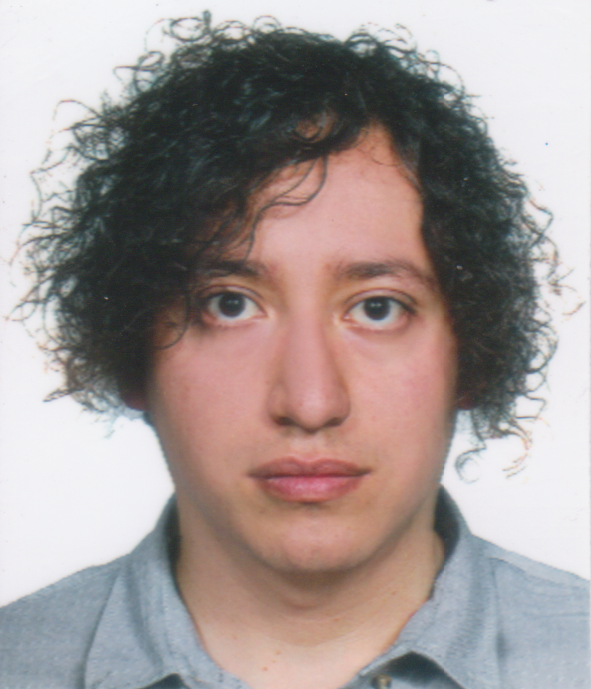
\includegraphics[width=2.5cm]{Images/fotoinfantil.png}}

\section{Descripción Personal}

Aprendí a programar a lo largo de mi carrera en Física, principalmente en temas de análisis numérico, ya que me interesa la investigación en el área de la relatividad numérica. Sin embargo, fui descubriendo áreas tales como deep learning y análisis de datos que pronto captaron mi interés, por lo que decidí realizar una maestría en ciencias de la computación. Sé utilizar sistemas GNU/Linux mediante la terminal y tengo conocimiento de varios lenguajes de programación. He trabajado principalmente en el ámbito académico, pero sé que también puedo sobresalir en el área empresarial, ya que estoy dispuesto a aprender más para así poder resolver todos los problemas de la vida real que puedan surgir.

\section{Datos Personales}

\begin{tabular}{rl}
%\textsc{Lugar y Fecha de Nacimiento:} & México | Septiembre 25, 1992 \\
\textsc{Dirección:} & Ciudad de México, México \\
\textsc{Teléfono:} & +52 5539347885\\
\textsc{email:} & \href{mailto:uzmar.gomez@ciencias.unam.mx}{uzmar.gomez@ciencias.unam.mx}\\
\textsc{LinkedIn:} & \href{www.linkedin.com}{www.linkedin.com/in/uzmargomez}\\
\textsc{Github:} & \href{https://github.com/uzmargomez}{https://github.com/uzmargomez}\\
\textsc{HackerRank:} & \href{https://www.hackerrank.com/uzmar_gomez}{https://www.hackerrank.com/uzmar\_gomez}\\
\textsc{Documentos Importantes:} & \href{https://www.dropbox.com/sh/bgvhqn1rrbzae7b/AAB4xslXKE_fjft6BQ5SR8D8a?dl=0}{Carpeta Dropbox}\\
\end{tabular}

%----------------------------------------------------------------------------------------
%	EDUCATION
%----------------------------------------------------------------------------------------

\section{Educación}

\subsection*{Física}

\begin{tabular}{r|p{14.5cm}}	
	
%------------------------------------------------	
\begin{comment}
	
	\textsc{In Progress} & \textbf{Master of Science in \textsc{\large{Physics}}}, Deparment of Physics \& Astronomy, University of British Columbia (UBC), \small British Columbia, Canada.\\
	\textsc{2019} & \small Advisor: \\
	& \\
	&\normalsize \textsc{Current Overall Score}: /10\hyperlink{grdsmscphysics}{\hfill | \footnotesize Detailed List of Grades}\\
	\multicolumn{2}{c}{}\\
	
\end{comment}	
%------------------------------------------------	
	
	\textsc{2018} & \textbf{Licenciado en \textsc{\large{Física}}}, Facultad de Ciencias, Universidad Nacional Autónoma de México (UNAM), \small Ciudad de México, México.\\
	\textsc{2011} & Tesis: \emph{``Estudio Numérico de la Ecuación de Vlasov en la Métrica de Schwarzschild''}\\
	&\small Descripción: Se usaron esquemas en diferencias finitas que evolucionan la ecuación de Vlasov\\
	&\hspace{1.7cm} \small relativista en una métrica de agujero negro de fondo, asumiendo que esta es una\\
	&\hspace{1.7cm} \small ecuación advectiva con velocidades dependientes tanto del tiempo como del espacio.\\
	&\hspace{1.7cm} \small \\
	& \small Tutor: Dr. Miguel Alcubierre\\
	& \\
	&\normalsize \textsc{Promedio}: 9.37/10\hyperlink{grdsbach}{\hfill | \footnotesize Lista detallada de calificaciones}\\
	\multicolumn{2}{c}{}\\
	
%------------------------------------------------
	
\end{tabular}	

\subsection*{Ciencias de la Computación}

\begin{tabular}{r|p{14cm}}

%------------------------------------------------	
\begin{comment}	
	\textsc{Presente} & \textbf{Maestría en \textsc{\large{Ciencias de la Computación}}}, University of Illinois at Urbana-Champaign\\
	\textsc{2019}& \\
	\multicolumn{2}{c}{}\\
\end{comment}	

%------------------------------------------------		
	\textsc{2010} & \textbf{Carrera técnica en \textsc{\large{Computación}}}, ENP N\textsuperscript{\underline{o}} 7 Universidad Nacional Autónoma de México (UNAM), \small Ciudad de México, México.\\
	\textsc{2008}& \\
	&\normalsize \textsc{Promedio}: 9.1/10\hyperlink{grdstechcarr}{\hfill | \footnotesize Lista detallada de calificaciones}\\
	\multicolumn{2}{c}{}\\
	
%------------------------------------------------	
\end{tabular}

%----------------------------------------------------------------------------------------
%	COMPUTER SKILLS 
%---------------------------------------------------------------------------------------
\section{Habilidades Computacionales}

\begin{tabular}{r|p{10.5cm}}
	Lenguajes de Programación & Python, C/C++, Fortran, Julia, Go \\
	Machine/Deep Learning &  TensorFlow, Keras, PyTorch, Time Series analysis (Facebook Prophet), LDA, PCA, sistemas de recomendación, problemas de clasificación\\
	Web Frontend & HTML, Bootstrap \\
	Web Backend & Flask \\
	Sistemas Operativos & Debian GNU/Linux, Ubuntu GNU/Linux, Windows \\
	Contenedores & Docker, Kubernetes \\
	Bases de Datos& MySQL, MongoDB \\
	Control de Versiones & Git \\
	Computación en paralelo & CUDA C/C++, CUDA Python\\
	Visualización de datos & Tableu, PowerBI

%	\multicolumn{2}{c}{} \\
\end{tabular}


%----------------------------------------------------------------------------------------
%	LANGUAGES
%----------------------------------------------------------------------------------------

\section{Idiomas}

\begin{tabular}{rl}
	\textsc{Inglés} & Nivel B2, IELTS\\
	
	\textsc{Español} & Lengua Madre
\end{tabular}

%----------------------------------------------------------------------------------------
%	INTERESTS AND ACTIVITIES
%----------------------------------------------------------------------------------------

\section{Intereses y Actividades}

\subsection*{Académicas}
Ciencia de Datos, Machine Learning, Deep Learning, Análisis Numérico, Programación Competitiva, Relatividad General, Relatividad Numérica, Ondas Gravitacionales, Agujeros Negros, Mecánica Cuántica, Ciencias de la Computación, Electromagnetismo.
\subsection*{No Académicas}
Correr, Nadar, Tocar la Guitarra, Lectura de Ciencia Ficción y Fantasía, Viajar, Videojuegos. 

%----------------------------------------------------------------------------------------
%	PROFESSIONAL MEMBERSHIP
%----------------------------------------------------------------------------------------

\section{Membresías}

\begin{tabular}{r|l}
	\textsc{Sep 2019}& Miembro\\
	\textsc{Ene 2017}&\footnotesize{\textbf{Red Temática de Agujeros Negros y Ondas Gravitatorias (Red ANyOG, CONACYT).}}\\
	\multicolumn{2}{c}{} \\
	\textsc{Dic 2019}& Estudiante Asociado\\
	\textsc{Ene 2016}&\footnotesize{\textbf{Instituto de Ciencias Nucleares, UNAM.}}\\
	\multicolumn{2}{c}{} \\
	\textsc{Ene 2016} & Estudiante Asociado\\
	\textsc{Ene 2015}&\footnotesize{\textbf{Instituto de Física, UNAM.}}\\
	\multicolumn{2}{c}{} \\
\end{tabular}

%----------------------------------------------------------------------------------------
%	WORK EXPERIENCE 
%----------------------------------------------------------------------------------------

\section{Experiencia}
\bigskip

\subsection{Breve descripción}
\textbf{Dic 2019 - Presente}. He trabajado en un sistema de identificación de rostros basado en Álgebra Lineal y Redes Neuronales.

\textbf{Sep 2019 - Dic 2019}. Mi principal experiencia es como Trainee de Data Scientist en Softtek. Aprendí sobre diferentes técnicas estadísticas y de aprendizaje automático, así como algoritmos, para estudiar una amplia gama de problemas.

\textbf{2012 - 2019}. A lo largo de mi carrera he programado, principalmente en Python y C++, pero también en Julia, Matlab, etc., para diferentes propósitos, tales como realizar tareas y proyectos (en particular en las asignaturas de Física Computacional y Temas Selectos de Física Computacional). Como se menciona abajo, he impartido clases de Computación, en la cual se les enseñó el lenguaje de programación Python a estudiantes de Física. 

\textbf{2014 - 2015}. Ayudé en la administración de bases de datos del Laboratorio de Mecánica de la Facultad de Ingeniería en la UNAM, únicamente con el objetivo de aprender. Para este propósito se utilizaba SQL.

\textbf{Sep 2018 - Dic 2019}. Referente a la investigación, tengo experiencia utilizando el Einstein Toolkit, siendo este una plataforma de herramientas de software creada con el objetivo de avanzar y apoyar la investigación en astrofísica relativista y física gravitacional. Permite estudiar temas tales como el choque de agujeros negros, hidrodinámica relativista, etc. Esta herramienta, si bien está basada en C++ y Fortran, utiliza Python a manera de ensamblador de las diferentes piezas. 

\textbf{Feb 2019 - Jul 2019}. He utilizado Python, junto con sus herramientas TensorFlow y Keras, para clasificar galaxias usando la base de datos del Sloan Digital Sky Survey.

Relacionado a las asignaturas que he impartido:
\begin{itemize}
	\item Computación.
	
	\href{https://web.fciencias.unam.mx/asignaturas/102.pdf}{https://web.fciencias.unam.mx/asignaturas/102.pdf}

	\item Temas Selectos de Relatividad, Cosmología y Gravitación 1.
	
	\href{https://web.fciencias.unam.mx/docencia/horarios/presentacion/295997}{https://web.fciencias.unam.mx/docencia/horarios/presentacion/295997}
	
	\item Relatividad
	
	\href{https://web.fciencias.unam.mx/asignaturas/718.pdf}{https://web.fciencias.unam.mx/asignaturas/718.pdf}
	
	\item Matemáticas I para las Ciencias Aplicadas. 
	
	\href{http://www.fciencias.unam.mx/asignaturas/1118.pdf}{http://www.fciencias.unam.mx/asignaturas/1118.pdf}
	
	\item Matemáticas II para las Ciencias Aplicadas.
	
	\href{http://www.fciencias.unam.mx/asignaturas/1216.pdf}{http://www.fciencias.unam.mx/asignaturas/1216.pdf}
	

	
\end{itemize}

\subsection*{Técnica}

\begin{tabular}{r|p{13cm}}
	
	%------------------------------------------------
	
	\textsc{Dic 2019}& Trainee de Data Scientist en \textsc{Softtek}\\
	\textsc{Sep 2019}& \small Ciudad de México, México.\\
	\multicolumn{2}{c}{} \\
	
	%------------------------------------------------
	
	\textsc{Sep 2009}& Técnico en Computación en \textsc{Dirección General de Servicios a la Comunidad}\\
	\textsc{Jun 2009}& \small Ciudad de México, México.\\
	\multicolumn{2}{c}{} \\
	
	%------------------------------------------------
	
\end{tabular}


\subsection*{Vocacional}
\begin{tabular}{r|p{7.8cm}p{4cm}}
%------------------------------------------------

Semestre 2019-2 & Ayudante de Profesor B en \textsc{Facultad de Ciencias, UNAM} &\\
& \small Ciudad de México, México. & \\
& \footnotesize $\circ$ Matemáticas II para las Ciencias Aplicadas & | {\footnotesize M. en C. Alejandro Villarreal}\\
\multicolumn{3}{c}{} \\

%------------------------------------------------

Semestre 2019-1 & Ayudante de Profesor B en \textsc{Facultad de Ciencias, UNAM} &\\
& \small Ciudad de México, México. & \\
& \footnotesize $\circ$ Temas Selectos de Relatividad, Cosmología y Gravitación 1 & | {\footnotesize Dr. Miguel Alcubierre}\\
& \footnotesize $\circ$ Matemáticas I para las Ciencias Aplicadas & | {\footnotesize M. en C. Alejandro Villarreal}\\
\multicolumn{3}{c}{} \\

%------------------------------------------------

Semestre 2018-2 & Ayudante de Profesor B en \textsc{Facultad de Ciencias, UNAM} &\\
& \small Ciudad de México, México. & \\
& \footnotesize $\circ$ Relatividad & | {\footnotesize Dr. Miguel Alcubierre}\\
& \footnotesize $\circ$ Matemáticas II para las Ciencias Aplicadas & | {\footnotesize M. en C. Alejandro Villarreal}\\
\multicolumn{3}{c}{} \\

%------------------------------------------------

Semestre 2018-1 & Ayudante de Profesor B en \textsc{Facultad de Ciencias, UNAM} &\\
&\small Ciudad de México, México. & \\
& \footnotesize $\circ$ Relatividad & | {\footnotesize Dr. Miguel Alcubierre}\\
& \footnotesize $\circ$ Matemáticas I para las Ciencias Aplicadas & | {\footnotesize M. en C. Alejandro Villarreal}\\
\multicolumn{3}{c}{} \\

%------------------------------------------------
\end{tabular}

\begin{tabular}{r|p{7.8cm}p{4cm}}
Semestre 2017-2 & Ayudante de Profesor A en \textsc{Facultad de Ciencias, UNAM} &\\
&\small Ciudad de México, México. & \\
& \footnotesize $\circ$ Matemáticas II para las Ciencias Aplicadas & | {\footnotesize M. en C. Alejandro Villarreal}\\
\multicolumn{3}{c}{} \\

%------------------------------------------------

Semestre 2017-1 & Ayudante de Profesor A en \textsc{Facultad de Ciencias, UNAM} &\\
&\small Ciudad de México, México. & \\
& \footnotesize $\circ$ Matemáticas I para las Ciencias Aplicadas & | {\footnotesize M. en C. Alejandro Villarreal}\\
& \footnotesize $\circ$ Computación & | {\footnotesize M. en C. Alejandro Villarreal}\\
\multicolumn{3}{c}{} \\

%------------------------------------------------
\textsc{Jun 2017} & Profesor en \textsc{Coordinación de Programas de Atención Diferenciada para Alumnos, UNAM} &\\
& \small Ciudad de México, México. & \\
& \footnotesize $\circ$ Electrodinámica con una introducción a Relatividad Especial & | {\footnotesize Ing. Raúl Puente}\\
\multicolumn{3}{c}{} \\

%------------------------------------------------

Semestre 2016-1 & Ayudante de Profesor A en \textsc{Facultad de Ciencias, UNAM} &\\
& \small Ciudad de México, México. & \\
& \footnotesize $\circ$ Matemáticas I para las Ciencias Aplicadas & | {\footnotesize M. en C. Alejandro Villarreal}\\
\multicolumn{3}{c}{} \\
%------------------------------------------------
\end{tabular}

%----------------------------------------------------------------------------------------
%	CONFERENCES, SUMMER SCHOOLS AND WORKSHOPS ASSISTED
%----------------------------------------------------------------------------------------

\section{Conferencias, Cursos, Escuelas y Talleres}

\subsection*{Ciencias de la Computación}

\begin{tabular}{r|p{11cm}}
	
	\textsc{Mar 26, 2020} & \small \textbf{Especialización}. \textit{Accelerated Computer Science Fundamentals} (COURSERA)\\
	\textsc{Ago 04, 2019} & \small University of Illinois at Urbana-Champaign\\
	&\url{https://www.coursera.org/account/accomplishments/specialization/certificate/DRF2CVM7P7FB}\\
	\multicolumn{2}{c}{} \\
	
	%------------------------------------------------
	\textsc{Mar 26, 2020} & \small \textbf{Curso}. \textit{Unordered Data Structures} (COURSERA)\\
	\textsc{Sep 15, 2019} & \small University of Illinois at Urbana-Champaign\\
	&\url{https://www.coursera.org/account/accomplishments/certificate/DFHE5FBHVAAD}\\
	\multicolumn{2}{c}{} \\
	
	%------------------------------------------------
	\textsc{Mar 04, 2020} & \small \textbf{Curso}. \textit{Python Statistics for Data Science Course} (EDUREKA)\\
	\textsc{Feb 10, 2020} & \small Edureka! For Business\\
	&\url{https://www.edureka.co/lms/certificate/8a0976c4e21d5bee00ff053e2d8e3f3e}\\
	\multicolumn{2}{c}{} \\
	
	%------------------------------------------------

	\textsc{Sep 15, 2019} & \small \textbf{Curso}. \textit{Ordered Data Structures} (COURSERA)\\
	\textsc{Ago 11, 2019} & \small University of Illinois at Urbana-Champaign\\
	&\url{https://www.coursera.org/account/accomplishments/certificate/PZ9NABHA7XBY}\\
	\multicolumn{2}{c}{} \\
	
	%------------------------------------------------
	
	\textsc{Ago 11, 2019} & \small \textbf{Curso}. \textit{Object-Oriented Data Structures in C++} (COURSERA)\\
	\textsc{Ago 04, 2019} & \small University of Illinois at Urbana-Champaign\\
	&\url{https://www.coursera.org/account/accomplishments/certificate/2YKURK8TJJ5B}\\
	\multicolumn{2}{c}{} \\
	
	%------------------------------------------------
	
	\textsc{Jul 29, 2019} & \small \textbf{Curso}. \textit{Algorithmic Toolbox} (COURSERA)\\
	\textsc{Jun 02, 2019} & \small University of California San Diego, National Research University Higher School of Economics\\
	&\url{https://www.coursera.org/account/accomplishments/certificate/FBZ5SK3E9BB6}\\
	\multicolumn{2}{c}{} \\
	
	%------------------------------------------------
	
	\textsc{Apr 17, 2019} & \small \textbf{Curso}. \textit{Operating Systems and You: Becoming a Power User} (COURSERA)\\
	\textsc{Abr 03, 2019} & \small Grow with Google, Ciudad de México, México.\\
	&\url{https://www.coursera.org/account/accomplishments/certificate/V6STDES4HLPE}\\
	\multicolumn{2}{c}{} \\
	
	%------------------------------------------------
	
	\textsc{Mar 10, 2019} & \small \textbf{Curso}. \textit{Python Data Structures} (COURSERA)\\
	\textsc{Mar 08, 2019} & \small University of Michingan, Michigan, Estados Unidos.\\
	&\url{https://www.coursera.org/account/accomplishments/certificate/L6Y7MZQDAJHP}\\
	\multicolumn{2}{c}{} \\
	
	%------------------------------------------------
	
	\textsc{Feb 26, 2019} & \small \textbf{Curso}. \textit{Programming for Everybody (Getting Started with Python)} (COURSERA)\\
	\textsc{Feb 21, 2019} & \small Universidad de Michingan, Michigan, Estados Unidos.\\
	&\url{https://www.coursera.org/account/accomplishments/certificate/CNNYCJB5YB46}\\
	\multicolumn{2}{c}{} \\
	
	%------------------------------------------------
	
	\textsc{Feb 14, 2019} & \small \textbf{Curso}. \textit{Technical Support Fundamentals} (COURSERA)\\
	\textsc{Feb 03, 2019} & \small Grow with Google, Ciudad de México, México.\\
	&\url{https://www.coursera.org/account/accomplishments/certificate/YQRPQLC86CUM}\\
	\multicolumn{2}{c}{} \\
	
	%------------------------------------------------
	
	\textsc{Feb 5, 2019} & \small \textbf{Curso}. \textit{Introducción a Data Science: Programación Estadística con R} (COURSERA)\\
	\textsc{Feb 3, 2019} & \small Universidad Nacional Autónoma de México, Ciudad de México, México\\
	&\url{https://www.coursera.org/account/accomplishments/certificate/E75DVAG2956T}\\
	\multicolumn{2}{c}{} \\
	
	%------------------------------------------------
	
	\textsc{Jun 13, 2018} & \small \textbf{Escuela}. \textit{Deep Learning and Multimessenger Astronomy}\\
	\textsc{Jun 9, 2018} & \small Tecnológico de Monterrey, Guadalajara, México.\\
	\multicolumn{2}{c}{} \\
	
	%------------------------------------------------
	
	\textsc{Ene 27, 2017} & \small \textbf{Curso}. \textit{Linux Básico}\\
	\textsc{Ene 16, 2017} & \small Facultad de Ingeniería UNAM, Ciudad de México, México.\\
	\multicolumn{2}{c}{} \\
	
	%------------------------------------------------
	
	\textsc{Jul 01, 2016} & \small \textbf{Curso}. \textit{Fundamentos de Fortran}\\
	\textsc{Jun 20, 2016} & \small Facultad de Ingeniería UNAM, Ciudad de México, México.\\
	\multicolumn{2}{c}{} \\
	
	%------------------------------------------------
	
\end{tabular}

\subsection*{Física}
\begin{tabular}{r|p{11cm}}
	%------------------------------------------------
	
	\textsc{Nov 11, 2018} & \small \textbf{Escuela}. \textit{Tercera Reunión de la Red Temática de Agujeros Negros y Ondas Gravitatorias}\\
	\textsc{Nov 9, 2018} &\small Playa del Carmen, Quintana Roo, México.\\
	\multicolumn{2}{c}{} \\
	
	%------------------------------------------------
	
	\textsc{Nov 9, 2018} & \small \textbf{Escuela}. \textit{Tercera Escuela de Relatividad General y Ondas Gravitatorias, Doceava Escuela de la División de Gravitación y Física Matemática}\\
	\textsc{Nov 5, 2018} &\small Playa del Carmen, Quintana Roo, México.\\
	\multicolumn{2}{c}{} \\
	
	%------------------------------------------------
	
	\textsc{Ago 12, 2017} & \small \textbf{Taller}. \textit{Quinto Taller de Gravitación y Cosmología.}\\
	\textsc{Ago 10, 2017} & \small Instituto de Ciencias Físicas UNAM, Cuernavaca, México.\\
	\multicolumn{2}{c}{} \\
	
	%------------------------------------------------
	
	\textsc{Ago 9, 2017} & \small \textbf{Escuela}. \textit{Segunda Escuela de Relatividad y Ondas Gravitatorias}\\
	\textsc{Ago 7, 2017} & \small Instituto de Ciencias Físicas UNAM, Cuernavaca, México.\\
	\multicolumn{2}{c}{} \\
	
	%------------------------------------------------
	
	\textsc{Ene 18, 2016} & \small \textbf{Curso}. \textit{Introducción a la Electrodinámica Relativista}\\
	\textsc{Ene 7, 2016} & \small Facultad de Ingeniería UNAM, Ciudad de México, México.\\
	\multicolumn{2}{c}{} \\
	
	%------------------------------------------------
\end{tabular}

%----------------------------------------------------------------------------------------
%	VOLUNTEER ACTIVITIES
%----------------------------------------------------------------------------------------

\section{Actividades Voluntarias}

\begin{tabular}{r|p{11cm}}

	%------------------------------------------------	
	
	\textsc{Sep 2019} & Profesor\\
	\textsc{Mar 2019} &\footnotesize{\textbf{Consejo Estudiantil Universitario (CEU México)}}\\
	&\footnotesize{Dotar a los universitarios de herramientas que contribuyan a desarrollar sus habilidades académicas. profesionales y personales, a fin de facilitar su inserción laboral y la definición de su proyecto de vida.}\\
	\multicolumn{2}{c}{} \\	
	
	%------------------------------------------------	
	
	\textsc{Mar 2019} & Voluntario\\
	\textsc{Sep 2018} &\footnotesize{\textbf{Programa Adopta Un Talento (PAUTA)}}\\
	&\footnotesize{Fomentar las vocaciones científicas de manera que los niños y adolescentes a los que les gusta la ciencia, así como aquellos con aptitudes sobresalientes, encuentren un espacio donde puedan compartir su interés por la misma y desarrollen habilidades que les permitan potencializar su vocación científica.}\\
	\multicolumn{2}{c}{} \\
	
	%------------------------------------------------		

\end{tabular}

%----------------------------------------------------------------------------------------
%	PRESENTATIONS AT CONFERENCES AND POSTER SESSIONS
%----------------------------------------------------------------------------------------

\section{Presentaciones y Pósters}

\begin{tabular}{r|p{11cm}}
	%------------------------------------------------
	
	\textsc{Oct 11, 2017} & Póster en \textsc{LX Congreso Nacional de Física}\\
	 &\small Monterrey, México\\
	&\footnotesize{Presenté un póster sobre mi tesis ``Estudio Numérico de la Ecuación de Vlasov en la Métrica de Schwarzschild''.}\\
	\multicolumn{2}{c}{} \\
	
	%------------------------------------------------
\end{tabular}



%----------------------------------------------------------------------------------------
%	SCHOLARSHIPS AND ADDITIONAL INFO
%----------------------------------------------------------------------------------------

\section{Becas, premios, honores y logros.}

\begin{tabular}{r|l}
\textsc{2017} & Beca otorgada por Conclusión de Proyecto\\
\textsc{2016}&\footnotesize{\textbf{Programa de Apoyo a Proyectos de Investigación e Innovación Tecnológica (PAPIIT)}.}\\
\multicolumn{2}{c}{} \\
\textsc{2016} & Beca otorgada por Conclusión de Licenciatura\\
\textsc{2015} &\footnotesize{\textbf{Programa de Apoyo a Proyectos de Investigación e Innovación Tecnológica (PAPIIT)}.}
\end{tabular}

%----------------------------------------------------------------------------------------
%	PUBLICATIONS
%----------------------------------------------------------------------------------------
\begin{comment}
\section{Publications}
\end{comment}

%----------------------------------------------------------------------------------------
%	REFERENCES
%----------------------------------------------------------------------------------------

\section{Referencias}
\small
\begin{tabular}{rl}
	\textsc{Nombre:} & Ing. Raúl Puente Mancilla \\
	\textsc{Institución:} & Facultad de Ingeniería, UNAM.\\
	\textsc{Ocupación:} & Profesor, Administrador de Base de Datos\\
	\textsc{email:} & \href{mailto:raulpuente@fisica.unam.mx}{raulpuente@fisica.unam.mx}\\
	\multicolumn{2}{c}{} \\
	\textsc{Nombre:} & M. en C. Alejandro Villarreal \\
	\textsc{Institución:} & Facultad de Ciencias, UNAM.\\
	\textsc{Ocupación:} & Investigador, Profesor\\
	\textsc{email:} & \href{mailto:alejandro.v@ciencias.unam.mx}{alejandro.v@ciencias.unam.mx}\\
	\multicolumn{2}{c}{} \\	\textsc{Nombre:} & Dr. Miguel Alcubierre \\
	\textsc{Institución:} & Instituto de Ciencias Nucleares, UNAM.\\
	\textsc{Ocupación:} & Director, Investigador, Profesor\\
	\textsc{email:} & \href{mailto:malcubi@nucleares.unam.mx}{malcubi@nucleares.unam.mx}\\
	\multicolumn{2}{c}{} \\
	\begin{comment}
	\textsc{Name:} & Eng. Raúl Puente \\
	\textsc{Institution Name:} & Institute of Physics, UNAM.\\
	\textsc{Occupation:} & Researcher\\
	\textsc{email:} & \href{mailto:raulpuente@fisica.unam.mx}{raulpuente@fisica.unam.mx}\\
	\multicolumn{2}{c}{} \\
	\end{comment}
\end{tabular}
\begin{center}
	\textsc{Actualizado \today}
\end{center}


\newpage

%----------------------------------------------------------------------------------------
%	GRADE TABLES
%----------------------------------------------------------------------------------------
\begin{comment}
\par{\centering\LARGE \hypertarget{grdsmscphysics}{Master of Science in \textsc{Physics}}\par}\par{\centering\Large University of British Columbia (UBC)\par}\large{\centering Grades\par}\small
\bigskip
\bigskip
\bigskip
\begin{center}
	\begin{tabular}{lc}
		\multicolumn{1}{c}{\textsc{Course}} & \textsc{Grade}\\ \hline \\
		I &  \\ 
		O &  \\ \\
		
		\textsc{Overall Score}&\textbf{9.1}
	\end{tabular}
\end{center}
\vspace{3cm}
%------------------------------------------------


\par{\centering\LARGE \hypertarget{grdsmsccompscience}{Master of Science in \textsc{Computer Science}}\par}\par{\centering\Large University of Illinois at Urbana-Champaign (UIUC)\par}\large{\centering Grades\par}\small
\bigskip
\bigskip
\bigskip
\begin{center}
	\begin{tabular}{lc}
		\multicolumn{1}{c}{\textsc{Course}} & \textsc{Grade}\\ \hline \\
		I &  \\ 
		O &  \\ \\
		
		\textsc{Overall Score}&\textbf{9.1}
	\end{tabular}
\end{center}
\vspace{3cm}
%------------------------------------------------
\end{comment}
\newpage
\par{\centering\LARGE \hypertarget{grdsbach}{Licenciatura en \textsc{Física}}\par}\par{\centering\Large Universidad Nacional Autónoma de México (UNAM)\par}\large{\centering Calificaciones\par}\small
\bigskip
\bigskip
\bigskip
\begin{center}
\begin{tabular}{lcc}
\multicolumn{1}{c}{\textsc{Asignatura}} & \textsc{Calificación}&\textsc{Créditos}\\ \hline \\
Cálculo Diferencial e Integral I & 07 & 18\\
Álgebra & 10 & 10\\
Computación & 10 & 6\\
Geometría Analítica I & 08 & 10\\
Cálculo Diferencial e Integral II & 10 & 18\\ 
Física Contemporánea & 09 & 6\\
Mecánica Vectorial & 9 & 12\\ 
Geometría Analítica II & 09 & 10\\
Laboratorio de Mecánica & 10 & 6\\
Fenómenos Colectivos & 10 & 12\\
Laboratorio de Fenómenos Colectivos & 09 & 6\\
Álgebra Lineal I & 10 & 10\\ 
Ecuaciones Diferenciales I & 08 & 10\\
Óptica & 09 & 12\\
Álgebra Lineal II & 10 & 10\\
Cálculo Diferencial e Integral III & 07 & 18\\
Electromagnetismo I & 9 & 12\\
Laboratorio de Electromagnetismo & 10 & 6\\
Cálculo Tensorial & 9 & 10\\
Cálculo Diferencial e Integral IV & 07 & 18\\
Introducción a la Física Cuántica & 10 & 12\\
Laboratorio de Óptica & 10 & 6\\
Termodinámica & 09 & 12\\
Matemáticas Avanzadas de la Física & 10 & 10\\
Física Computacional & 10 & 12\\
Mecánica Cuántica & 09 & 12\\
Variable Compleja I & 10 & 10\\
Temas Selectos de Física Matemática y Teórica I & 10 & 6\\
Electromagnetismo II & 08 & 12\\
Laboratorio de Electrónica & 10 & 6\\
Física Estadística & 10 &12\\
Laboratorio de Física Contemporánea I & 10 & 6\\
Variable Compleja II & 10 & 10\\
Mecánica Analítica & 10 & 12\\
Relatividad & 09 & 06\\
Introducción a la Física de Partículas Elementales I & 10 & 06\\
Dinámica de Medios Deformables & 10 & 12\\
Física Atómica y Materia Condensada & 09 & 06\\
Física Nuclear y Subnuclear & 09 & 06\\
Laboratorio de Física Contemporánea II & 10 & 06\\
Topología y Geometría Diferencial para Físicos & 10 & 06\\
Temas Selectos de Relatividad Cosmología y Gravitación I & 10 & 06\\
Temas Selectos de Física Computacional I & 10 & 06\\ \\
Inglés & AC &	00\\ \\
& Créditos Totales & 418\\ \\
&\textsc{Promedio}&\textbf{9.37}
\end{tabular}
\end{center}
\vspace{5cm}

%------------------------------------------------


\par{\centering\LARGE \hypertarget{grdstechcarr}{Carrera Técnica en \textsc{Computación}}\par}\par{\centering\Large Universidad Nacional Autónoma de México (UNAM)\par}\large{\centering Calificaciones\par}\small
\bigskip
\bigskip
\bigskip
\begin{center}
	\begin{tabular}{lc}
		\multicolumn{1}{c}{\textsc{Asignatura}} & \textsc{Calificación}\\ \hline \\
		Introducción a la Computación & 9 \\ 
		Sistemas Operativos & 10 \\
		Aplicaciones de Uso General & 9 \\
		Solución de Problemas y Técnicas de Programación & 9 \\
		Programación Estructurada & 10 \\
		Programación Orientada a Eventos & 9 \\
		Análisis y Diseño de Sistemas & 10 \\
		Programación Orientada a Bases de Datos & 6 \\
		Redes de Área Local & 9 \\
		Mantenimiento Preventivo y Correcciones Menores para PC's & 10 \\ \\

		\textsc{Promedio}&\textbf{9.1}
	\end{tabular}
\end{center}

%------------------------------------------------
\begin{comment}
\bigskip

\par{\centering\Large \hypertarget{grds_usc}{Exchange Program at \textsc{usc}, Los Angeles}\par}\large{\centering Grades\par}\normalsize

\begin{center}
\begin{tabular}{lcc}
\multicolumn{1}{c}{\textsc{Exam}} & \textsc{Grade} & \textsc{Grade Points}\\ 
\hline
Corporate Financial Strategy & A & 4\\
Derivatives & A & 4\\
Money, Credit, and Banking & A & 4\\
Business Strategy & A- & 3.5\\
& &\\\cline{2-3}
& \textsc{Gpa} & \textbf{3.875}
\end{tabular}
\end{center}

\end{comment}

%----------------------------------------------------------------------------------------

\end{document}
